\chapter{Analisis}
\label{chap:analisis}

\section{Analisis Permainan \textit{Snake} yang Sudah Ada}
Permainan \textit{Snake} yang akan dianalisis adalah \textit{Slither.io}. Slither.io adalah permainan \textit{web} yang dapat dimainkan oleh lebih dari 1 pemain(\textit{multiplayer}). Cara bermainya mirip seperti permainan \textit{Snake} pada umumnya yaitu ular harus memakan makanan untuk mendapatkan skor. Dalam permainan ini, setiap pemain berkompetisi untuk menjadi pemain terbaik dengan cara mendapatkan skor sebanyak-banyaknya. Pemain akan kalah apabila ular milik pemain menabrak ular milik pemain lain. 

\subsection{Ular dan Makanan}
Ular pada \textit{Slither.io} dibentuk dengan menggunakan sekumpulan lingkaran yang saling berdempetan satu sama lain seperti pada Gambar~\ref{fig:slitherUlar}. Bagian kepala pada ular ditandai menggunakan sepasang mata. Ketika memakan makanan, tubuh ular akan memanjang dengan menambahkan sebuah lingkaran pada bagian ekor ular. Setiap memulai permainan, tubuh ular akan memiliki warna yang ditentukan secara acak.\\

Makanan pada \textit{Slither.io} berbentuk lingkaran. Makanan ini ada yang berukuran besar dan ada yang berukuran kecil. Makanan ini tersebar pada labirin, jumlahnya sangat banyak dan warnanya bermacam-macam. Gambar~\ref{fig:slitherMakanan} merupakan sekumpulan makanan yang terdapat pada labirin. Setiap makanan akan menambah skor sebanyak 1 poin.

\begin{figure}[H]
	\centering  
	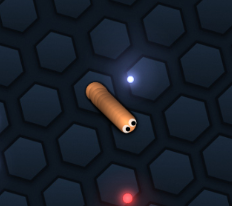
\includegraphics[scale=0.7]{slitherUlar}  
	\caption[Ular pada \textit{Silther.io}]{Ular pada \textit{Silther.io}}
	\label{fig:slitherUlar} 
\end{figure}

\begin{figure}[H]
	\centering  
	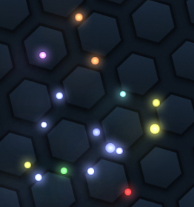
\includegraphics[scale=0.7]{slitherMakanan}  
	\caption[Makanan pada \textit{Slither.io}]{Makanan pada \textit{Slither.io}}
	\label{fig:slitherMakanan} 
\end{figure}

\subsection{Pergerakan Ular}
Ular pada \textit{Slither.io} digerakan dengan menggunakan keyboard dan \textit{mouse}. Tombol ke kiri akan membuat ular bergerak berlawanan arah jarum jam dan tombol ke kanan akan membuat ular bergerak searah jarum jam. Semakin lama tombol ditekan, maka ular akan berbelok lebih cepat. Kursor pada \textit{mouse} membuat ular bergerak ke arah posisi kursor tersebut. Ular dapat melaju dengan cepat(\textit{speed up}) dengan menekan tombol \textit{mouse} kiri seperti yang terdapat pada Gambar~\ref{fig:slitherSpeed}. Ketika ular sedang melaju dengan cepat, total skor yang didapat akan berkurang. 

\begin{figure}[H]
	\centering  
	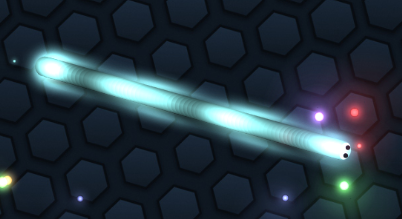
\includegraphics[scale=0.7]{slitherSpeed}  
	\caption[Ular sedang melaju dengan cepat(\textit{speed up})]{Ular sedang melaju dengan cepat(\textit{speed up})}
	\label{fig:slitherSpeed} 
\end{figure}

\subsection{Labirin}
Labirin pada \textit{Slither.io} hanya ada 1 saja. Labirin ini berbentuk lingkaran yang sisinya merupakan dinding. Apabila ular menabrak dinding labirin, maka permainan akan berakhir. Labirin ini cukup besar sehingga sangat kecil kemungkinan ular untuk menabrak dinding labirin. Gambar~\ref{fig:slitherLabirin} menunjukan peta labirin pada \textit{Slither.io}. Pada peta labirin tersebut terdapat sekumpulan titik bewarna abu-abu yang merepresentasikan makanan.

\begin{figure}[H]
	\centering  
	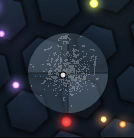
\includegraphics[scale=1]{slitherLabirin}  
	\caption[Peta labirin pada \textit{Slither.io}]{Peta labirin pada \textit{Slither.io}}
	\label{fig:slitherLabirin} 
\end{figure}

\section{Analisis Sistem yang Dibangun}
Permainan \textit{Snake} 360 yang akan dibangun memiliki cara bermain yang mirip seperti permainan Snake pada umumnya. Perbedaan antara \textit{Snake} 360 dengan permainan \textit{Snake} pada umumnya adalah \textit{Snake} 360 dapat menambahkan level dan labirin sendiri. 

\subsection{Menggambar Ular dan Apel}
Tubuh ular dibuat menggunakan sekumpulan \textit{line}/garis pendek. Setiap bagian tubuh ular memiliki panjang sebesar 1 \textit{pixel} dan lebar tubuhnya sebesar 5 \textit{pixel}. Bagian tubuh ular dibuat pendek untuk memudahkan pengecekan jika terjadi ular menabrak tubuhnya sendiri. Untuk lebar ular, disesuaikan dengan besar apel yaitu 10 \textit{pixel}. Setiap bagian tubuh ular memiliki koordinat masing-masing. Koordinat setiap bagian tubuh disimpan pada sebuah \textit{array} agar menggambar ular menjadi lebih mudah. Dalam tahap ini, tubuh ular masih berupa sekumpulan titik-titik yang merupakan koordinat bagian tubuh ular seperti pada Gambar~\ref{fig:titikUlar}. Algoritma untuk menggambar ular adalah dengan mengambil koordinat bagian tubuh ular mulai dari elemen \textit{array} paling pertama(arr[0]) dan elemen \textit{array} selanjutnya(arr[1]) lalu buat garis yang \textit{start point}nya adalah elemen pertama(arr[0]) dan \textit{end point}nya adalah elemen \textit{array} kedua(arr[1]). Setelah itu ambil koordinat elemen \textit{array} yang merupakan \textit{end point} pada garis sebelumnya(arr[1]) dengan elemen \textit{array} selanjutnya(arr[2]) dan gambar garisnya. Lakukan hal tersebut sampai \textit{end point} garis mencapai elemen \textit{array} paling akhir. Setelah digambar maka ular akan terlihat seperti Gambar~\ref{fig:garisUlar}.

\begin{figure}[H]
	\centering  
	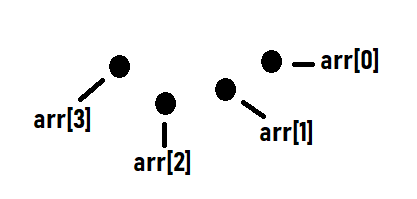
\includegraphics[scale=0.7]{titikUlar}  
	\caption[Koordinat bagian tubuh ular pada \textit{array}]{Koordinat bagian tubuh ular pada \textit{array}}
	\label{fig:titikUlar} 
\end{figure}

\begin{figure}[H]
	\centering  
	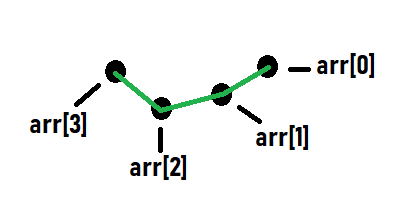
\includegraphics[scale=0.7]{garisUlar}  
	\caption[Tubuh ular setelah digambar menggunakan garis]{Tubuh ular setelah digambar menggunakan garis}
	\label{fig:garisUlar} 
\end{figure}

Untuk membuat apel digunakan \textit{quadratic B\'ezier curve}. Kurva ini digunakan untuk membuat bagian-bagian apel yang melengkung. Bagian tersebut ditandai dengan lingkaran bewarna merah seperti yang ditunjukan pada Gambar~\ref{fig:apel}(gambar diambil dari pinterest. Link:https://www.pinterest.com/pin/690317449105509454/).

\begin{figure}[H]
	\centering  
	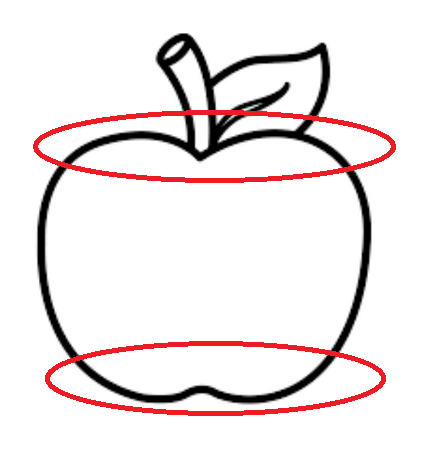
\includegraphics[scale=0.5]{apel}  
	\caption[Bagian pada apel(lingkaran merah) yang akan dibuat menggunakan kurva]{Bagian pada apel(lingkaran merah) yang akan dibuat menggunakan kurva}
	\label{fig:apel} 
\end{figure}

Pertama, tentukan besar apel yang ingin dibuat. Dalam permainan ini besar apel yang dibuat adalah 10 pixel. Besar apel dibuat lebih besar dari lebar ular karena jika besar apel sama dengan lebar ular, besar apel terlihat sangat kecil. Selain itu, apel ini digambar pada layout yang berbentuk persegi. Layout persegi ini juga dapat mempermudah penggambaran apel. Karena menggunakan layout persegi, maka origin terletak pada titik sudut di sebelah kiri atas. Setelah itu, gambar setiap bagian apel. Bagian apel dibagi menjadi 4 seperti pada Gambar~\ref{fig:apel2} sehingga besar setiap bagian apel tersebut adalah 5 pixel. 

\begin{figure}[H]
	\centering  
	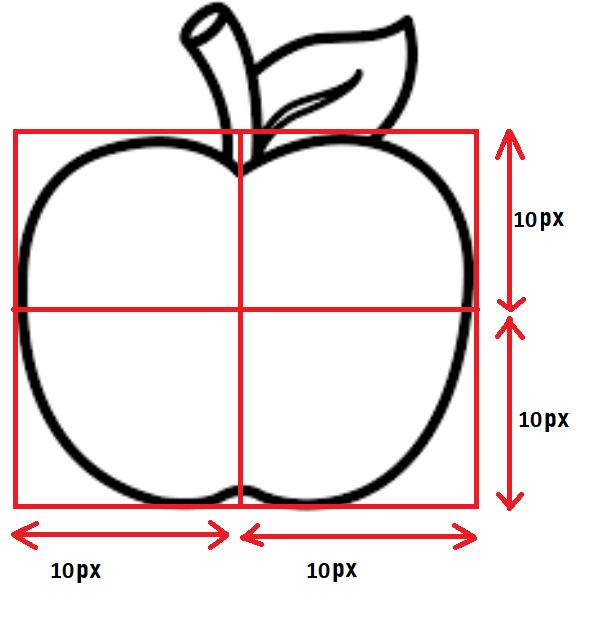
\includegraphics[scale=0.4]{apel2}  
	\caption[Pembagian gambar apel dengan layout persegi beserta ukuran pada setiap bagian]{Pembagian gambar apel dengan layout persegi beserta ukuran pada setiap bagian}
	\label{fig:apel2} 
\end{figure}

Gambar bagian atas apel terlebih dahulu. Gunakan method moveTo() untuk menentukan titik mulainya. Titik mulainya terletak pada bagian tengah atas apel yang melengkung ke dalam. Dari titik itu, buat kurva yang control pointnya adalah titik ujung layout persegi. Jika ingin menggambar bagian kiri apel terlebih dahulu maka control pointnya adalah titik ujung kiri layout tersebut. Setelah itu, tentukan end point kurva tersebut. Pada Gambar~\ref{fig:apel3} terdapat start point, control point dan end point untuk membuat bagian sisi kiri atas apel. Sesudah itu, buatlah bagian bawah apel. Caranya sama seperti sebelumnya namun control pointnya dan end pointnya berbeda. Posisi control pointnya sedikit menjorok ke dalam dan posisi end pointnya terdapat di tengah bawah seperti pada Gambar~\ref{fig:apel4}. Start point tidak perlu diatur lagi, karena start pointnya sudah tergantikan dengan posisi end point pada kurva sebelumnya. Sampai pada bagian ini, bagian kiri apel sudah selesai dibuat. Untuk membuat bagian kanan apel, caranya sama seperti membuat bagian kiri apel. Karena bagian kiri apel simetris dengan bagian kanan apel, maka hanya perlu mengubah control point dan end pointnya saja. Dengan memanfaatkan bentuk simetris dari apel, maka jarak antara control point dan end point pada bagian kiri apel dengan batasan tengah sama dengan jarak antara control point dan end point dengan batas tengah pada bagian kanan apel. 

\begin{figure}[H]
	\centering  
	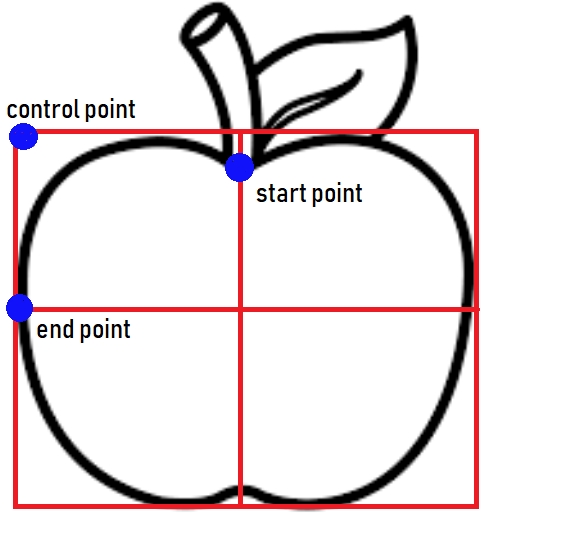
\includegraphics[scale=0.4]{apel3}  
	\caption[Start point, control point dan end point untuk menggambar apel bagian kiri atas]{Start point, control point dan end point untuk menggambar apel bagian kiri atas}
	\label{fig:apel3} 
\end{figure}

\begin{figure}[H]
	\centering  
	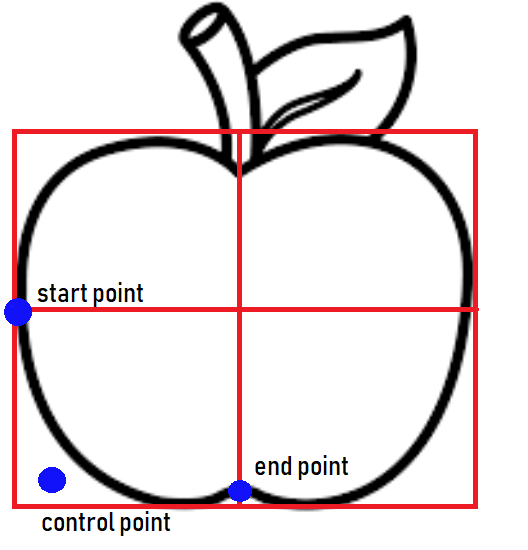
\includegraphics[scale=0.4]{apel4}  
	\caption[Start point, control point dan end point untuk menggambar apel bagian kiri bawah]{Start point, control point dan end point untuk menggambar apel bagian kiri bawah}
	\label{fig:apel4} 
\end{figure}

\subsection{Pergerakan Ular}
Untuk membuat ular bergerak maju, dilakukan penambahan kepala dan pembuangan ekor secara bersamaan ketika ular sedang bergerak maju. Ilustrasinya dapat dilihat pada Gambar~\ref{fig:snakeMoveForward}. Untuk membuat ular bergerak dengan menggunakan cara pada Gambar~\ref{fig:snakeMoveForward}, algoritmanya adalah sebagai berikut : Pertama, semua elemen array akan dishift/digeser dan elemen pertama akan digantikan dengan koordinat yang baru. Setelah itu dilakukan pengecekan apakah panjang tubuh ular lebih besar dari jumlah elemen array tubuh ular. Jika benar, maka tidak dilakukan pembuangan elemen terakhir dan jika salah, maka tidak akan dilakukan apa-apa. 

\begin{figure}[H]
	\centering  
	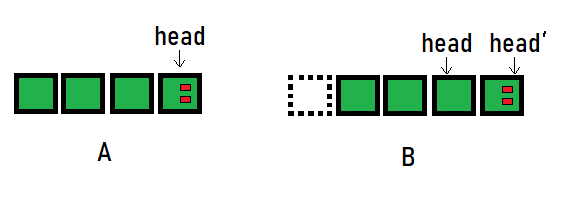
\includegraphics[scale=0.5]{snakeMoveForward}  
	\caption[Ilustrasi ular sebelum bergerak maju(A) dan setelah bergerak maju(B)]{Ilustrasi ular sebelum bergerak maju(A) dan setelah bergerak maju(B)}
	\label{fig:snakeMoveForward} 
\end{figure}

Kecepatan ular pada permainan ini adalah 1 sampai 5 \textit{pixel per frame}. Kecepatan maksimal ular tidak boleh melebihi lebar tubuh ular. Jika kecepatanya melebihi lebar ular, maka ketika terjadi tabrakan dengan tubuhnya sendiri, kepala ular tidak akan bertabrakan dengan tubuhnya. Kepala ular akan terlihat seolah-olah melompati tubuhnya sendiri. Dalam permainan ini, kecepatan ular adalah 2 \textit{pixel per frame}, karena dengan kecepatan 1 \textit{pixel per frame}, ular terlihat bergerak lebih lambat.\\

Ular dapat berbelok dengan menggunakan tombol pada \textit{keyboard}. Tombol ke kiri akan membuat ular bergerak melawan arah jarum jam dan tombol ke kanan akan membuat ular akan bergerak searah jarum jam. Pada permainan yang akan dibuat ini, digunakan sudut sebagai nilai untuk membuat ular dapat bergerak 360$^\circ$. Jika menekan tombol ke kiri maka sudut akan berkurang dan jika menekan tombol ke kanan maka sudut akan bertambah. Ketika menambahkan dan mengurangi sudut, perlu dilakukan pengecekan apabila nilai sudut valid atau tidak. Karena nilai sudut yang valid adalah antara nilai 0 sampai 360, maka apabila nilai sudut kurang dari 0, ubahlah sudut tersebut menjadi 360 dan apabila nilai sudut lebih besar dari 360, ubahlah nilai sudut tersebut menjadi 0. Dibutuhkan rumus trigonometri untuk menentukan posisi kepala ular. Untuk menghitung posisi koordinat x, digunakan \textit{sinus} sedangkan untuk menghitung posisi koordinat y menggunakan \textit{cosinus}. Jadi koordinat x dan y pada kepala ular akan ditambahkan dengan hasil perhitungan \textit{sinus} dan \textit{cosinus}.

\subsection{Labirin}
Dinding labirin akan dibuat dengan menggunakan garis. Cara pembuatanya sama dengan membuat tubuh ular yaitu dengan menggunakan titik-titik yang dihubungkan dengan garis yang pendek. Dinding labirin dapat juga dibuat dengan menggunakan kurva dikarenakan pergerakan ular yang sudah dapat bergerak 360$^\circ$. Level pada labirin dapat ditentukan berdasarkan kerumitan labirin. Labirin yang memiliki dinding yang banyak dan kompleks akan mendapatkan level yang lebih tinggi dibandingkan dengan labirin yang memiliki sedikit dinding dan lebih simpel. 

\subsection{Pengecekan tabrakan(\textit{Collision Detection})}
Pada permainan ini terdapat pengecekan tabrakan yang dapat mengecek apakah ular sudah memakan makanan, ular menabrak tubuhnya sendiri, dan ular menabrak dinding labirin. Seluruh pengecekan ini akan dilakukan pada setiap \textit{frame}. Pada pengecekan tabrakan pada apel dan ular, hanya perlu mengecek tabrakan antara kepala ular dengan apel. Karena jalur yang dilalui oleh kepala ular, akan selalu dilalui oleh bagian tubuh ular. Dengan kata lain, bagian tubuh ular akan mengikuti ke mana kepala ular akan bergerak. Dengan ini, tidak perlu dilakukan \textit{collision detection} antara bagian tubuh ular dengan apel. Cukup hanya dengan mengecek tabrakan antara kepala ular dengan apel saja. Untuk mengetahui terjadinya tabrakan antara ular dengan apel, maka akan dibuat daerah tabrakan pada apel. Daerah tabrakan ini digunakan untuk mengecek apakah 2 benda saling bertabrakan satu sama lain. Daerah tabrakan pada apel ditandai dengan arsiran bewarna merah yang terdapat pada Gambar~\ref{fig:apelArsir}. Namun, untuk membuat daerah tabrakan ini cukup sulit ketika mengecek adanya tabrakan antara ular dengan apel terutama pada bagian lengkungan pada apel. Karena itu, daerah tabrakan pada apel dibuat dengan menggunakan bentuk persegi seperti pada Gambar~\ref{fig:apelArsirPersegi}. Jika posisi kepala ular berada di dalam daerah tabrakan apel, maka dipastikan bahwa ular tersebut sudah memakan apel. Algoritma untuk mengecek tabrakan adalah sebagai berikut : cek apakah koordinat x dari kepala ular lebih besar dari posisi sisi kiri daerah tabrakan dan lebih kecil dari posisi sisi kanan daerah tabrakan. Kemudian cek apakah koordinat y dari kepala ular lebih besar dari posisi sisi atas daerah tabrakan dan lebih kecil dari posisi sisi bawah daerah tabrakan. Jika posisi kepala ular berada memenuhi ketentuan tersebut, maka kepala ular berada di dalam daerah tabrakan apel.\\

\begin{figure}[H]
	\centering  
	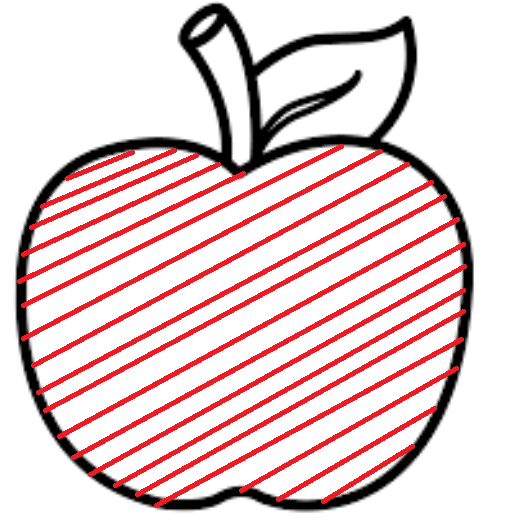
\includegraphics[scale=0.4]{apelArsir}  
	\caption[Daerah tabrakan pada apel]{Daerah tabrakan pada apel}
	\label{fig:apelArsir} 
\end{figure}

\begin{figure}[H]
	\centering  
	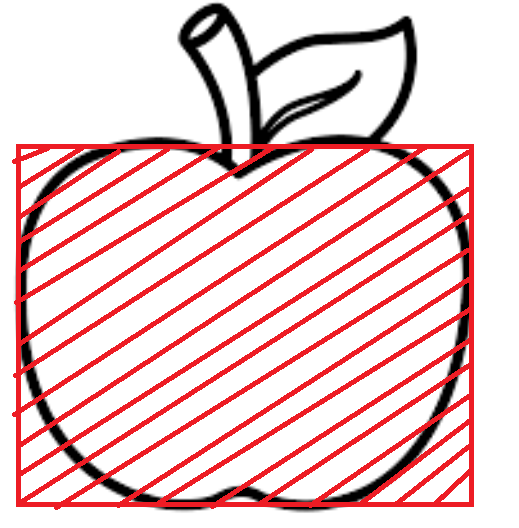
\includegraphics[scale=0.4]{apelArsirPersegi}  
	\caption[Daerah tabrakan berbentuk persegi pada apel]{Daerah tabrakan berbentuk persegi pada apel}
	\label{fig:apelArsirPersegi} 
\end{figure}

Untuk mengecek tabrakan antara ular dengan tubuhnya sendiri adalah dengan mengecek tabrakan antara kepala ular dengan seluruh bagian tubuh ular. Algoritma pengecekanya adalah sebagai berikut : jika koordinat x kepala ular lebih kecil dari koordinat x bagian tubuh ular dikurangi panjang dari bagian tubuh ular dan lebih besar dari koordinat x bagian tubuh ular ditambah dengan panjang dari bagian tubuh ular. Kemudian dicek apabila koordinat y kepala ular lebih kecil dari koordinat y bagian tubuh ular dikurangi panjang dari bagian tubuh ular dan lebih besar dari koordinat y bagian tubuh ular ditambah dengan panjang dari bagian tubuh ular. Apabila posisi kepala ular memenuhi ketentuan tersebut, maka posisi kepala ular berada di dalam daerah tabrakan pada sebuah bagian tubuh ular. \\

Untuk mengecek tabrakan dengan labirin, algoritmanya sama dengan mengecek tabrakan antara ular dengan tubuh ular. Karena cara pembuatan labirin sama hampir sama dengan cara pembuatan tubuh ular, maka dilakukan pengecekan antara kepala ular dengan setiap dinding labirinya.

\section{Analisis Berorientasi Objek}

\subsection{Skenario Permainan}
Pada bagian ini akan dijelaskan dan ditunjukkan diagram \textit{use case} dari permainan \textit{Snake} 360. Penjelasan meliputi skenario, aktor, prakondisi skenario normal dan eksepsi. Aktor yang melakukanya adalah pemain. Pada Gambar~\ref{fig:useCase} terdapat diagram \textit{use case} dari permainan \textit{Snake} 360.

\begin{figure}[H]
	\centering  
	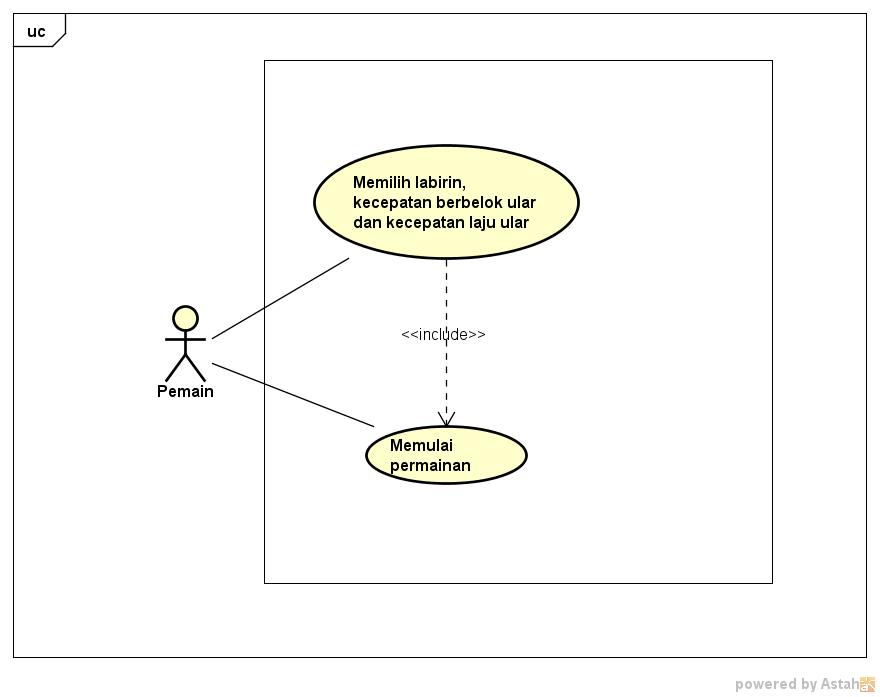
\includegraphics[scale=0.4]{useCase}  
	\caption[Diagram \textit{use case} dari permainan \textit{Snake} 360]{Diagram \textit{use case} dari permainan \textit{Snake} 360}
	\label{fig:useCase} 
\end{figure}

Berikut adalah skenario dari diagram \textit{use case} :

\begin{enumerate}
	\item Skenario : Mulai bermain \\
Aktor : Pemain \\
Prakondisi : Pemain memulai permainan.\\
Skenario normal : Pemain memulai bermain. Setelah memilih, pemain akan memilih level dan labirin. \\
Eksepsi : - \\

	\item Skenario : Memilih level dan labirin \\
Aktor : Pemain \\
Prakondisi : Pemain sudah mulai bermain. \\
Skenario normal : Pemain memilih level dan labirin yang diinginkan. \\ 
Eksepsi : - \\
\end{enumerate}

\subsection{Diagram Kelas}
Pada Gambar~\ref{fig:classDiagram} terdapat diagram kelas dari \textit{Snake} 360.

\begin{figure}[H]
	\centering  
	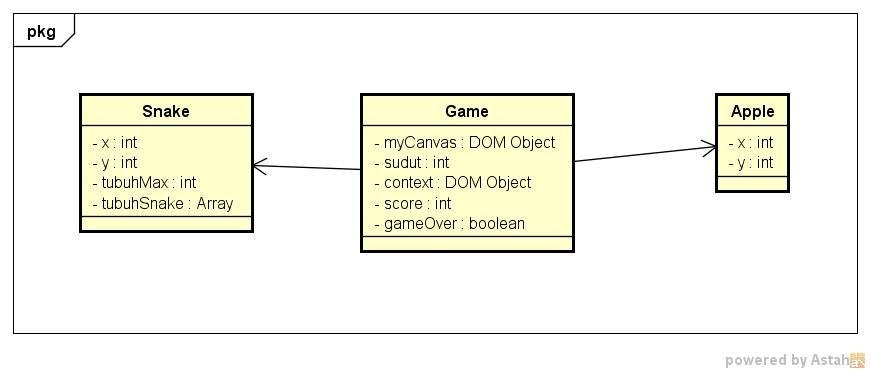
\includegraphics[scale=0.4]{classDiagram}  
	\caption[Diagram class dari permainan \textit{Snake} 360]{Diagram kelas dari permainan \textit{Snake} 360}
	\label{fig:classDiagram} 
\end{figure}

Diagram kelas terdiri dari beberapa kelas yaitu :

\begin{enumerate}
	\item Kelas Snake merupakan  kelas yang merepresentasikan objek ular.
	\item Kelas Apel merupakan kelas yang merepresentasikan objek apel.
	\item Kelas Game merupakan kelas yang mengatur jalanya permainan.
\end{enumerate}

Berikut adalah atribut yang dimiliki setiap kelas :

\begin{enumerate}
	\item Kelas Snake\\
\textbf{int}

\begin{itemize}
	\item x, merupakan posisi ular pada koordinat x
	\item y, merupakan posisi ular pada koordinat y
	\item tubuhMax, merupakan panjang tubuh ular
\end{itemize}

	\item Kelas Apel\\
	\textbf{int}
	
\begin{itemize}
	\item x, merupakan posisi apel pada koordinat x
	\item y, merupakan posisi apel pada koordinat y
\end{itemize}

\item Kelas Game \\
\textbf{int}

\begin{itemize}
	\item sudut, merupakan besar sudut yang digunakan untuk ular berbelok.
	\item score, merupakan skor yang didapat pada permainan.
\end{itemize}

\textbf{boolean}
\begin{itemize}
	\item gameOver, memberitahu apakah permainan sudah berakhir atau belum.
\end{itemize}

\end{enumerate}